% ===========================================================================
% Physical AI Systems, cover and title pages
% ===========================================================================
%
% Loaded after tex/preamble.tex, which defines the palette this file uses.
% This file draws; the preamble configures. Keep it that way.
%
% \maketitle produces two pages:
%
%   1. The cover. Full-bleed ETH blue, crimson rules top and bottom, and the
%      proposal-permission loop drawn as the book's signature diagram. The
%      loop is on the cover because it is the argument: an untrusted proposer,
%      a trusted permitter, an irreversible world, and the feedback that makes
%      the whole thing endogenous.
%   2. The title page. Quiet, typographic, no artwork.
%
% Text on the cover is set here rather than pulled from \@title so the cover
% can be composed as a piece of design. If the book is retitled, change it in
% both places.
%
% ===========================================================================

\makeatletter
\renewcommand*{\maketitle}{%

% --- Page 1: cover ---------------------------------------------------------
\begin{titlepage}\thispagestyle{empty}%
  \newgeometry{margin=0pt}%
  % Measure natural width of "Machine Learning Systems" at 43.5pt for perfect margin symmetry
  \newlength{\mlsysTitleLen}%
  \newlength{\mlsysLeftM}%
  \newlength{\mlsysRightM}%
  \settowidth{\mlsysTitleLen}{{\fontsize{43.5pt}{43.5pt}\selectfont Machine Learning Systems}}%
  \setlength{\mlsysLeftM}{0.5\dimexpr\paperwidth - \mlsysTitleLen\relax}%
  \setlength{\mlsysRightM}{\dimexpr\mlsysLeftM + \mlsysTitleLen\relax}%
  \begin{tikzpicture}[remember picture,overlay]

    % Pure white background
    \fill[white] (current page.south west) rectangle (current page.north east);

    % Floating 3D sculpture artwork in upper canvas (Candidate 4 / Gyroscopic Gimbal)
    \node[anchor=center, inner sep=0pt] at ([xshift=0.55in, yshift=1.50in]current page.center) {%
      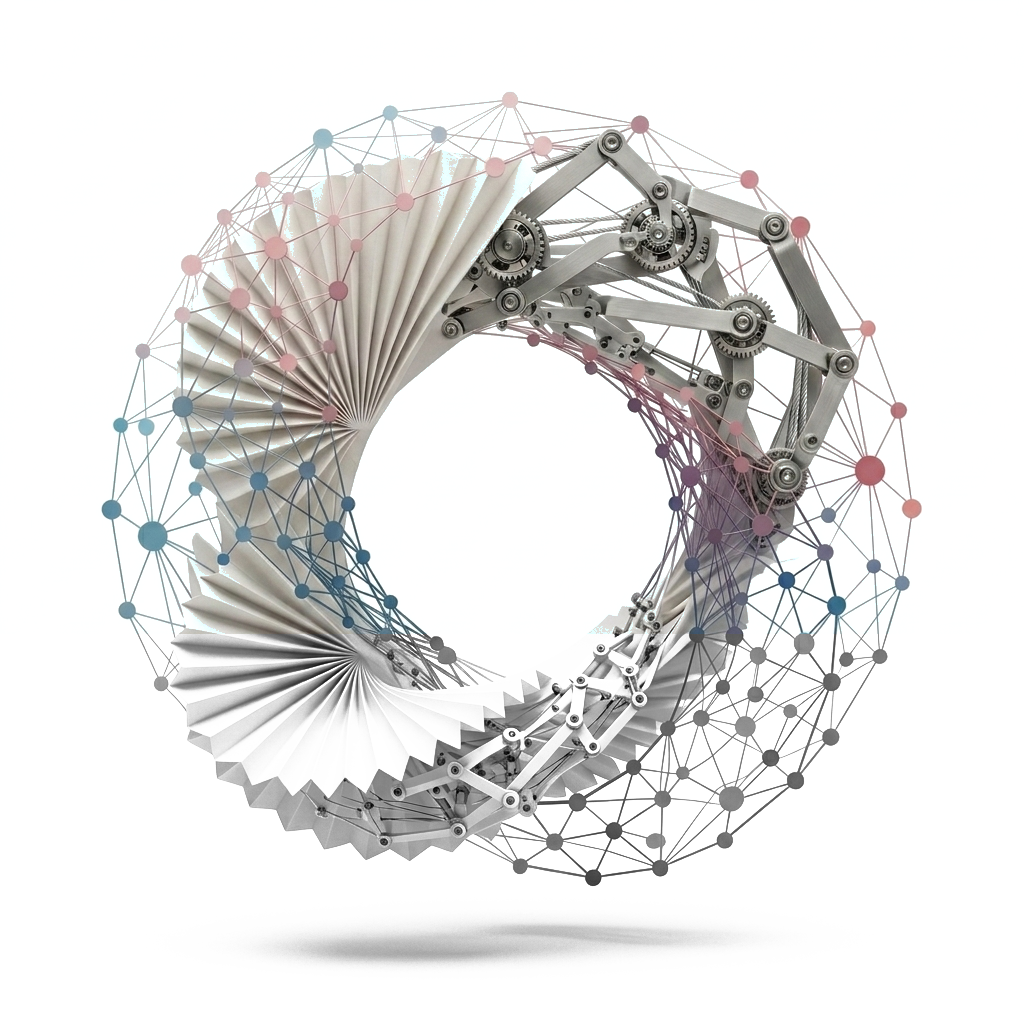
\includegraphics[width=0.96\paperwidth]{assets/covers/cover-physical-robotic-finger-loop-art.png}%
    };

    % Left-aligned Subtitle aligned to exact left edge of Title (MIT Press Calibrated y=2.40in)
    \node[anchor=south west, inner sep=0pt] at ([xshift=\mlsysLeftM, yshift=2.40in]current page.south west) {%
      {\fontsize{23.5pt}{27.5pt}\rmfamily\selectfont\color{ink}Physical AI}%
    };

    % Single-Line Main Title (MIT Press Calibrated y=1.62in)
    \node[anchor=south west, inner sep=0pt] at ([xshift=\mlsysLeftM, yshift=1.62in]current page.south west) {%
      {\fontsize{44pt}{48pt}\rmfamily\selectfont\color{ink}Machine Learning Systems}%
    };

    % Single-Line Right-aligned Author (MIT Press Calibrated y=0.78in)
    \node[anchor=south east, inner sep=0pt] at ([xshift=\mlsysRightM, yshift=0.78in]current page.south west) {%
      {\fontsize{21.5pt}{25pt}\rmfamily\selectfont\color{ink}Vijay Janapa Reddi}%
    };

  \end{tikzpicture}%
  \restoregeometry
\end{titlepage}%

% --- Page 2: interior title page (Matching Volume 1 & Volume 2) ---------
\begin{titlepage}\thispagestyle{empty}%
  \raggedright
  \vspace*{-0.6\topskip}

  {\fontsize{15pt}{17pt}\rmfamily\selectfont Physical AI: Machine Learning Systems\par}
  \vspace{0.8\baselineskip}
  {\fontsize{12pt}{14pt}\rmfamily\itshape\color{accentcolor}That Sense and Act\par}

  \vspace{10\baselineskip}

  {\fontsize{14pt}{16pt}\rmfamily\selectfont Vijay Janapa Reddi\par}
  \vspace{0.4\baselineskip}
  {\fontsize{10pt}{12pt}\rmfamily\selectfont\color{softink}Harvard University \ $\cdot$\  ETH Zurich\par}

  \vfill

  {\fontsize{11pt}{13pt}\rmfamily\selectfont%
   The MIT Press\\[0.4ex]%
   Cambridge, Massachusetts\\[0.4ex]%
   London, England%
  \par}

  \vspace*{0.02\textheight}
\end{titlepage}%

}
\makeatother
